%!TEX root = ../thesis.tex
\chapter{Introduction} \label{ch:introduction}
\section{Overview}
\subsection{Early artificial intelligence references}
Since ancient times, the human being has dreamed of artificial intelligence (AI). One of the first existing records dates back to \textit{Aristotle} (384–322 BCE) in his book \textit{Politics}, where the author imagined machines that would think by themselves and act autonomously, with the purpose of allowing humans enjoy leisure. In 10-70 CE, the mathematician and engineer \textit{Hero of Alexandria} designed several ancient automatons, one of the most famous was an automated theater that would play short performances in front of the audience.

In the 9th century, the three Persian brothers known as the \textit{Banū Mūsā} wrote the book of Ingenious Devices, where they illustrated hundreds of automatons along with other mechanical devices (timing and delay devices, automated valves, etc.) and described how to use them.

In the middle ages, the philosopher, scientist and bishop \textit{Albert Magnus} (13th century) manufactured several automatons. One of the most famous was a talking head that was able to imitate human voice and breadth. Later on, in the renaissance (15th century), the polymath \textit{Leonardo da Vinci} designed various automatons. His mechanical knight, is one of the first anthropomorphous automatons we have record of. This automaton was able to perform basic human-like motions through a system of pulleys and cables. Modern history represented the golden era of automatons. One of the most famous creators was the watchmaker \textit{Pierre Jaquet-Droz} (18th century), who built a number of automatons, including a three-year-old child that could write any letter of the alphabet. Other significant important creators of the era were \textit{Wolfgang von Kempelen} (1734-1804), who built \textit{the Turk}, an automaton that could beat any human at chess\footnote{Although after his death, it was discovered that it was actually nothing more than an automaton operated by a person from inside a wooden cabinet }, and \textit{Jacques de Vaucanson} (1709-1782), who built a number of automatons, including a duck that could eat and drink. Despite the complexity and ingenuity of these automatons, they were all purely mechanical and human operated, without any form of artificial intelligence.

There are also historical references to artificial intelligence in form of fiction stories. In \textit{The city of brass}, one of the tales included into the \textit{One Thousand and One Nights} (around the 10th century), the protagonist, a thief, comes across a city ruled by a wizard who created a brass anthropomorphic automaton that could talk and move like a human. In the 19th century, \textit{E.T.A. Hoffmann} (1776-1822) wrote the story \textit{The Sandman}, where the protagonist falls in love with an automaton created by a professor, without realizing she was actually a machine, and then suffering a mental breakdown when he found out. This automaton, known as Olympia, was able to move, talk and sing. In the novel \textit{Frankenstein} writen by \textit{Mary Shelley} in 1818, the scientist \textit{Victor Frankenstein} creates a human-like creature out of body parts of different people. Although, strictly speaking, this creature is not a machine, it is often seen as one of the first examples of intelligent creation.

The first recorded use of the term \textit{robot} was in the play \textit{R.U.R.} (\textit{Rossum’s Universal Robots}) by the Czech writer \textit{Karel Čapek} (1920), in which robots are manufactured as slaves to do the manual labor that humans do not want to do. This play is often seen as the beginning of the science fiction genre.

In 1941, the science fiction writer \textit{Isaac Asimov} published a short story called \textit{Runaround}, in which he introduced the three laws of robotics (depicted below), which are still used today as the basis for the ethical design of robots.


\begin{enumerate}

	\item A robot may not injure a human being or, through inaction, allow a human being to come to harm.

	\item A robot must obey the orders given to it by human beings, except where such orders would conflict with the First Law.

	\item A robot must protect its own existence as long as such protection does not conflict with the First or Second Law.

\end{enumerate}

The artificial intelligence dream has come and gone in waves over the years, but it has never lost its appeal to the human imagination. Each time a new wave of artificial intelligence hits, it brings with it renewed hope for the possibility that machines can think and act by themselves. However, it has not been until recently that artificial intelligence has begun to show significant promise for actually becoming a reality.

\subsection{Modern Artificial Intelligence}
In the 20th century, the AI dream started to become a reality with the development of the first computers. The idea of artificial intelligence was rediscovered in the 1950s, when \textit{Alan Mathison Turing} (1912 - 1954) — today known as the father of computer science — after secretly defeating the German intelligence's cryptography system (\textit{Enigma} machines) \autocite{Hodges:2000} and providing a proof showing that a general solution for the the \textit{Hilbert's Entscheidungsproblem} (an important symbolic logic challenge) was impossible \autocite{turing1936}, published the article entitled \textit{Computing Machinery and Intelligence} \autocite{turing1950} in which he described a game as a measure of machine intelligence. The currently known as \textit{Turing test} consists of a human interrogator trying to determine, by asking a series of questions, whether the entity it is talking to is a human or a machine. If the interrogator cannot tell the difference (70\% of the times after multiple 5 minutes conversations), then the machine is said to have passed the test.

\begin{figure}
	\centering
	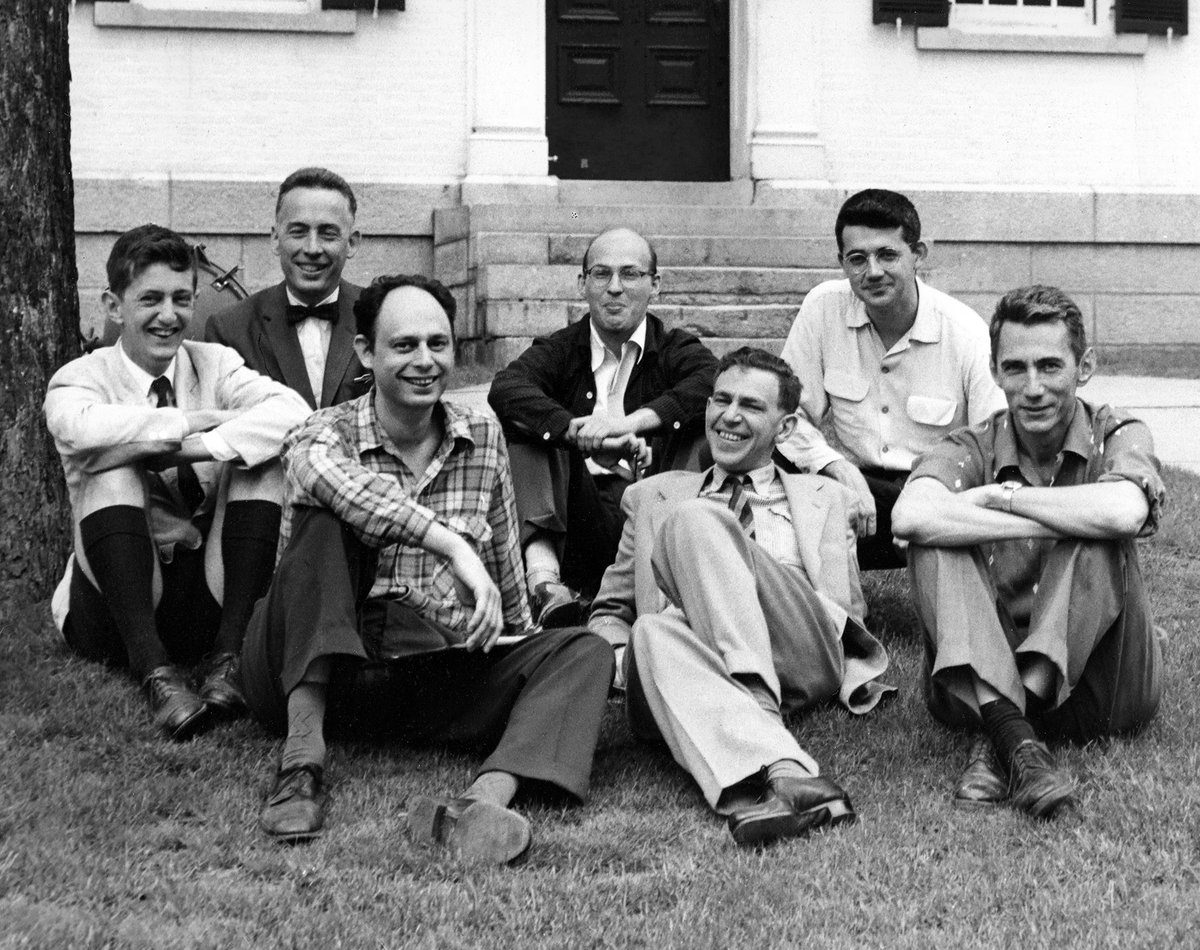
\includegraphics[width=.6\textwidth]{chapter1/images/dartmouth}
	\caption{\textit{Marvin Minsky}, \textit{John McCarthy}, \textit{Claude Shannon}, \textit{Ray Solomonoff} and other scientists at the \textit{Dartmouth Summer Research Project on Artificial Intelligence}}
	\label{fig:dartmouth_photo}
\end{figure}

The ``artificial intelligence'' term was not coined until 1956, when \textit{John McCarthy} (1927 - 2011) \textit{Nathaniel Rochester} (1919 - 2001) and \textit{Claude Shannon} (1916 – 2001) gave a conference at \textit{Dartmouth College}, in which the \textit{Dartmouth Summer Research Project on Artificial Intelligence} was proposed: a 2 month workshop that was organized to fund the artificial intelligence as an academic discipline (see the picture in figure \ref{fig:dartmouth_photo}). The project was funded by the \textit{United States Office of Naval Research}, and brought together some of the most prominent computer scientists of the time, including \textit{Marvin Minsky} (1927–2016), \textit{Arthur L. Samuel} (1916–1990), \textit{Ray Solomonoff} (1926-2009) and \textit{John Nash} (1928-2015).

However, the recent development of artificial intelligence has not been a linear process, and there have been ups and downs along the way, with several so-called \textit{AI winters}. The \textit{first AI winter} took place in the late 1970s and early 1980s, when research on artificial intelligence came to a standstill. In 1974, \textit{Sir James Lighthill}, a well-known British scientist, published a report \autocite{lighthillReport} (currently known as \textit{the Lighthill report}) that concluded that artificial intelligence was a waste of time and money. This publication, together with the oversized expectations for artificial intelligence at the time \autocite{russellNorvig}, led to a decrease in funding for AI research. As a result, the field of artificial intelligence went into decline, stalling for several years.

After the first AI winter (in the late 80s), the field experienced a revival, when several companies started investing in the development of \textit{Expert Systems}: a rebranded form of artificial intelligence. Software and hardware companies such as \textit{Teknowledge} and \textit{LISP Machines Inc.} grew rapidly during this time in order to meet the rising demand for artificial intelligence technology. All that motivated the AI research community to continue with their work. One of the most remarkable inventions of that decade was the successful application of the \textit{backpropagation} algorithm to neural networks by \textit{David Rumelhart} and \textit{Geoffrey Hinton} in 1986 \autocite{hinton1986}, which revived the study of artificial neural networks. All this sudden success, together to the collapse of \textit{LISP Machines Inc.} in 1987, led to the \textit{second AI winter}.

The 1990s started with a renewed interest in artificial intelligence. Motivated by the increasingly computational power, machine learning algorithms started to be applied to a wider range of tasks \autocite{Tesauro:1995}. Many interesting applications were developed during that decade across several industries like medical diagnosis \autocite{declaris1991, Klein1991, punch1992, Cinar1999}, psychology \autocite{Dorrer1995, denby1999, Ogawa1999, Perlovsky1999}, finance and logistics \autocite{Lipshutz1991, Benaroch1991, Johnson1991, Falas1994} and many others \autocite{Smithers1993, Yoo1994, Mashaly1994, Koyma1998}. The most sounded event of the 1990s was the victory of the IBM super-computer \textit{Deep Blue} \autocite{Campbell2002} over \textit{Garry Kasparov}, the world chess champion.

The 21st century represents one of the most fruitful periods for artificial intelligence, with several major achievements in different areas. In 1998, \textit{Yann Lecun} and his collaborators published their work on Convolutional Neural Networks \autocite{lecun1999}, a fundamental advance in machine learning which has been widely used in computer vision and other fields. Further research in neural networks \autocite{hinton2006, hinton2012} gave birth to novel techniques that allowed us training deeper models, leading to a re-branding of neural networks as deep learning. In 2011, \textit{IBM's} artificial intelligence program \textit{Watson} won the quiz game \textit{Jeopardy!} against two of the best human players of all time. Research in neural networks gave birth to novel techniques that allowed researchers to train deeper models, leading to a re-branding of neural networks as deep learning. In 2012, \textit{AlexNet} \autocite{krizhevsky2012}, a deep learning model developed by \textit{Geoffrey Hinton} and his collaborators, achieved state-of-the-art performance on the \textit{ImageNet} classification task \autocite{ILSVRC15}, kickstarting the current deep learning revolution. In 2016, \textit{Google's} artificial intelligence program \textit{AlphaGo} \autocite{silver2016} defeated the world champion \textit{Lee Sedol} in \textit{the game of Go}, a feat that was considered impossible a few years earlier, by using \textit{Reinforcement Learning} algorithms. \textit{Alpha Go Zero}, the \textit{Alpha Go's} big brother, proved in 2017 to be more powerful than its predecessor while not needing human interaction to learn \autocite{Silver2017a, Silver2017b}. In 2016, \textit{DeepMind} researchers published \textit{WaveNet} \autocite{vanderoord2016} (used in the experiments described in chapter \ref{ch:tts}), a deep autoregressive model that was able to produce natural raw audio waveforms faithfully representing human speech. In 2017, \textit{Ashish Vaswani et. al} published the transformer \autocite{vaswani2017} (used in the experiments described in chapter \ref{ch:salesforecast}), an new architecture designed for sequence transduction task that allowed parallel training, as opposed to its sequence-to-sequence predecessors \autocite{sutskever2014}. In 2020, \textit{OpenAI} researchers published \textit{GPT-3} \autocite{brown2020}, a massive neural network with 175 billion parameters which was able to achieve strong performance on many NLP tasks. In 2021, \textit{AlphaFold} was published by \textit{DeepMind} researchers \autocite{Jumper2021} as a method for inferring the 3D structure of a biological protein based on its genetic sequence, representing one of the major contributions of artificial intelligence to scientific discovery. In addition to the mentioned achievements, many algorithms have been published in the generative modeling field. Generative adversarial networks \autocite{Goodfellow2014}, variational autoencoders \autocite{kingma2019}, normalizing flows \autocite{kingma2016, kobyzev} and diffusion models \autocite{Prafulla2021} are some of the most remarkable examples. These topics will be discussed in detail in section \ref{sec:generative}.

Many more advances have been made in artificial intelligence in the past few years, which has led to an increased interest in the technology from both the private and public sectors. However, the application of artificial intelligence to complicated and important tasks, still faces many challenges. This is where deep learning comes into play, as it has shown the ability to achieve state-of-the-art results on a wide range of tasks. Therefore, the development of democratized and low-resource deep learning applications is essential for the future of artificial intelligence. Several of the last advances in the deep learning research community report prohibitive amounts of computation needed to train deep learning models \autocite{silver2016, kechyn2018, brown2020, floridi2020}. \textit{Strubell et al.} \autocite{strubell2019} estimated the amount of $CO_2$ emissions from training a large transformer network to be equivalent to the emissions of 5 average cars during all their lifetime, or those of a human during 60 years. Research in low-resource deep learning \autocite{howard2017, Han2017, Gao2018, sanchez2020, so2021} has shown that the ability to train deep learning models with a low amount of computation is possible, and essential for the future of artificial intelligence, and for the health of our planet.


\section{Contributions}
This dissertation encompasses two contributions to the state of the art of the field of deep learning training methods, and three applications of deep learning algorithms to industry problems. All the contributions are related to the efficient use of computational resources. Each of these studies is written as a different chapter, following the style of an academic publication, as they were originally written with that purpose. All of them are either published or submitted to peer-reviewed journals or conferences

The first contribution (chapter \ref{ch:modulus}) proposes a new activation function for deep learning models. This activation function is the modulus function. This work shows that, in line with the current research trends, non-monotonic activation functions generally produce better results than monotonic ones. Additionally, the modulus activation function is very efficient to compute, as it consists of a single-bit operation, and its derivative (being either 1 or -1) has constant 1-norm. These properties are specially useful for embedded applications. Moreover, the results show that the proposed activation function achieves superior results in computer vision tasks when compared with the state of the art alternatives.

The second contribution (chapter \ref{ch:distillation}) proposes combining the knowledge of several large pretrained models in order to improve the performance of small low-resource pretrained models. The results of this work show that it is possible to significantly increase the accuracy of the smallest pretrained models, allowing for computational savings and improved performance.

Two of the applications covered in this thesis belong to the speech technology field. The former(chapter \ref{ch:kws}) studies how to build a \textit{Keyword Spotting} speech recognition system using an efficient version of a convolutional neural network. In this study, the proposed system is able to beat the performance of all the benchmarks found in the literature when tested against the most complex subtasks. This work has been published in the proceedings of \textit{European Symposium of Artificial Neural Networks (ESANN 2020)} \autocite{valles2021a}. The latter study (\ref{ch:tts}) proposes a standlalone state of the art \textit{Text-To-Speech} model capable of synthesizing intelligible voice in thousands of voice profiles, while generating speech with meaningful and expressive prosody variations. The proposed approach, removes the dependency of previous models on a production voice system, which makes it more efficient at training and inference time, and enables offline and on-device operations. This study was done as part of the work of the author at \textit{Alexa AI} and has been published in the proceedings of \textit{Interspeech 2020} conference \autocite{valles2021b}.

Finally, the last application covered in this thesis tackles the problem of sales forecasting in the field of logistics. Two end-to-end systems with two different deep learning techniques (sequence-to-sequence models and transformers) are proposed. The results of this work conclude that it is possible to build end to end systems to predict the sales of multiple individual products, at multiple points of sale and different times. The proposed model beats the state of the art alternatives found in the bibliography.

The unpublished works referenced in this section have already been submitted to a journal and, at the time of writing this paragraph, are under revision.

\section{Thesis structure}
This thesis is organized as follows. Chapter \ref{ch:background} covers the minimum background needed to understand the methods and algorithms applied in the following chapters. Chapter \ref{ch:modulus} proposes the modulus as activation function, showing its benefits over other alternatives. Chapter \ref{ch:distillation} studies how to combine pretrained models using knowledge distillation. Chapter \ref{ch:salesforecast} explores the application of sequence-to-sequence models and transformers to approach the sales forecasting problem, from an end-to-end perspective. Chapter \ref{ch:kws} presents an end-to-end keyword spotting system with convolutional networks. Chapter \ref{ch:tts} proposes a state-of-the-art multispeaker Text-To-Speech (TTS) system with prosody modeling. Finally, chapter \ref{ch:conclusions} wraps the general conclusions of the studies presented in the previous chapters.


% Todo: add references to my papers
% Todo: update current state of the papers